\chapter{Spatial Transformations for the Computations of the Log-composition: SE(2) and SVF}\label{ch:spatial_transformations}


\begin{flushright}
	\emph{Every working mathematician knows that if one does not control oneself (best of all by examples), then after some ten pages half of all the signs in formulae will be wrong and twos will find their way from denominators into numerators. \\ -V.I. Arnold}
\end{flushright}

In the previous chapter we have introduced some essential mathematical tools for the numerical computation of the log-composition. They can be applied for several groups of transformation. In this research we show how they behave on two selected groups:
\begin{enumerate}
	\item[$SE(2)$ -] The group of rigid body transformation of the plane (any combination of bi-dimensional rotations and translations) is the optimal playground to test the numerical methods introduced so far. Here all the closed form can be derived analytically, and therefore a ground truth is always available for comparisons. A representation of this Lie group as a subgroup of the real linear group $GL(2)$, with corresponding Lie algebra will be provided, with all of the closed form of the numerical computations presented in this research.
	\item[SVF -] The subgroup of the set of diffeomorphisms parametrized by SVF, is the second group used to test the numerical methods here presented for the computation of the log-composition. Each one can be applied for the composition of SVF in the diffeomorphic demons and for the log-demons. In this case we do not know any closed form, but if we consider an improper norm in the space of transformation we still have a method to compare SVF and assess the quality of the results.
\end{enumerate}

\noindent
Since each of the theoretical elements at the core of the Lie group theory, depends strongly on the transformations considered, in this chapter we will see how they can be applied for the cases of SE(2) and the Lie group of diffeomorphisms parametrized with stationary velocity fields.

\section{The Lie Group of Rigid Body Transformations}\label{se:rigid_body_transformations}
% group
Each element of the group of rigid body transformation (or euclidean group) $SE(2)$ can be computed as the consecutive application of a rotation and a translation applied to any point $(x,y)^T$ of the plane:
\begin{align*}
\left (  
\begin{array} {c }
X \\
Y
\end{array}
\right )  
= 
R(\theta)
\left (  
\begin{array} {c }
x \\
y
\end{array}
\right ) 
+
t
=
\left (
\begin{array} {c c }
\cos(\theta) & - \sin(\theta) \\
\sin(\theta) & \cos(\theta) 
\end{array}
\right )
\left (  
\begin{array} {c }
x \\
y
\end{array}
\right ) 
+
\left (  
\begin{array} {c }
t_x \\
t_y
\end{array}
\right ) 
\end{align*}
where the rotation matrix defined by $\theta$ belongs to the special orthogonal group $SO(2)$.\\
We can represent the elements of $SE(2)$ in two different form: as ternary vector (restricted form) 
\begin{align*}
SE(2)^{v} 
:=
\{ (\theta, t_x, t_y) \mid \theta \in [0, 2\pi),   t_x, t_y \in\mathbf{R}^2  \}
\end{align*}
or with matrices (matrix form)
\begin{align*}
SE(2) 
:= 
\left \{
\left (
\begin{array} {c c }
R(\theta) & t \\
0 & 1 
\end{array}
\right )
=
\left (
\begin{array} {c c c }
\cos(\theta) & - \sin(\theta)& t_{x} \\
\sin(\theta) & \cos(\theta) & t_{y}\\
0 & 0 &  1
\end{array}
\right )
\mid
\theta \in  [0, 2\pi), (t_x, t_y) \in\mathbf{R}^2
\right \}
\end{align*}
The group $SE(2)$ it is a manifold with a differentiable structure compatible with the operation of composition, whose Lie algebra is given in matrix form by (see \cite{hall2015lie, gallier2011geometric} for an introduction).
\begin{align*}
\mathfrak{se}(2) := 
\left \{
\left (
\begin{array} {c c }
dR(\theta) & dt \\
0 & 0
\end{array}
\right )
=
\left (
\begin{array} {c c c }
0 & -\theta &  dt_{x} \\
\theta & 0 & dt_{y} \\
0& 0 & 0
\end{array}
\right )
\mid
\theta \in  [0, 2\pi), (tx, ty) \in\mathbf{R}^2
\right \}
\end{align*}
and it is indicated with $\mathfrak{se}(2)^{v}$ in its vector form.\\

Given $r$, element of $SE(2)$ with $\theta\neq 0$. Its image with the Lie group logarithm is
\begin{align*}
\log(r)
&=
\sum_{k=1}^{\infty} (-1)^{k+1}~\frac{(r - I)^k}{k}
=
\left (
\begin{array} {c c }
dR(\theta) & L(\theta)t \\
0 & 1 
\end{array}
\right )
\\
&=
\left (
\begin{array} {c c c}
0   & - \theta& \frac{\theta}{2} (\frac{\sin(\theta)}{1-\cos(\theta)} t_x + t_y )\\
\theta & 0     & \frac{\theta}{2} (- t_x + \frac{\sin(\theta)}{1-\cos(\theta)} t_y )\\
0 & 0 &  0
\end{array}
\right )
\end{align*}
where therefore 
\begin{align*}
dR(\theta) = 
\left (
\begin{array} {c c }
0 & -\theta \\
\theta & 0 
\end{array}
\right )
\qquad \qquad 
L(\theta) = 
\frac{\theta}{2}
\left (
\begin{array} {c c }
\frac{\sin(\theta)}{1-\cos(\theta)} & 1 \\
-1 & \frac{\sin(\theta)}{1-\cos(\theta)}
\end{array}
\right )
\end{align*}
On the way back, the exponential of $dr \in \mathfrak{se}(2)$ is given by:
\begin{align*}
\exp(dr)
&=
\sum_{k=1}^{\infty} \frac{dr^{k}}{k!}
=
\left (
\begin{array} {c c }
R(\theta) & L(\theta)^{-1}t \\
0 & 1 
\end{array}
\right )
\\
&=
\left (
\begin{array} {c c c}
\cos(\theta)   & - \sin(\theta)& \frac{1}{\theta} (\sin(\theta)dt_x - (1-\cos(\theta)) dt_y )\\
\sin(\theta) & \cos(\theta)     & \frac{1}{\theta} (- (1-\cos(\theta))dt_x + \sin(\theta) dt_y )\\
0 & 0 &  1
\end{array}
\right )
\end{align*}
where
\begin{align*}
L(\theta)^{-1} = 
\frac{1}{\theta}
\left (
\begin{array} {c c }
\sin(\theta) & -(1-\cos(\theta)) \\
(1-\cos(\theta)) & \sin(\theta)
\end{array}
\right )
\end{align*}
When $\theta$ is zero, $R(\theta)$ and $dR(\theta)$ coincide with the identity, and the transformation results in a translation. For proof and further details see for example \cite{gallier2011geometric} \cite{hall2015lie}.\\

At this point it is important to notice that: 
\begin{enumerate}
	%infinite series 
	\item The infinite series of matrices  do not raises any theoretical issues, since the sum is defined in the group as subset of a bigger algebra that contains both the Lie group and the Lie algebra. The infinite series of matrices appears to be the natural way to back and forth from the group to the algebra. A second door to passing from one structure to the other, when $\mathbf{r}$ has a little rotation element appears to be provided by the following approximations:
	\begin{align*}
	\exp(r) \simeq I + r
	\qquad 
	\log(dr) \simeq dr - I
	\end{align*}
	In fact for little $\theta$, $\sin(\theta) \simeq \theta$, $\cos(\theta) \simeq 0 $ and $ L(\theta)^{-1} \simeq I$.
	% restriction of the domain.
	\item The map $\exp$ is not well defined over its whole domain $\mathfrak{se}(2)$. Given two elements $(\theta_0, dr_{0x}, dr_{0y})$ and $(\theta_1, dr_{1x}, dr_{1y})$, they have the same image with $\exp$ function if the two following conditions are both satisfied:
	\begin{enumerate}
		\item[i)] Exists an integer $k$ such that $\theta_0 = \theta_1 + 2k\pi$.
		\item[ii)] the translation $(dr_{0x}, dr_{0y})$ coincides with $(dr_{1x}, dr_{1y})$ up to a factor $\frac{\theta_0 \mod 2\pi}{\theta_1}$.
	\end{enumerate}
	To have a bijective correspondence we have to restrict the domain of $\exp$ to a space where if $\exp(\theta_0, dr_{0x},d t_0y) = \exp(\theta_1, dr_{1x}, dr_{1y})$ it implies  $(\theta_0, dr_{0x}, dr_{0y}) = (\theta_1, dr_{1x}, dr_{1y})$.
	It can be easy to prove that the sought space is the quotient of $\mathfrak{se}(2)$ over the equivalence relation $\sim$, defined as 
	\begin{align*}
		(\theta_0, dr_{0x}, dr_{0y} & ) \sim (\theta_1, dr_{1x}, dr_{1y})
		\\
		~^{\text{def}}&\iff
		\\
		\exists k\in\mathbb{Z} \mid \theta_0 = \theta_1 + 2k\pi 
		&~\text{ and }~
		(dr_{0x}, dr_{0y}) = \frac{\theta_0 \mod 2\pi}{\theta_1}(dr_{1x}, dr_{1y})
	\end{align*}
	The new algebra defined by the set of equivalence classes of this relation is indicated - with the standard convention, see \cite{artin2011algebra} - with $\mathfrak{se}(2)/\sim$. With this restriction of the domain$\exp$ is a bijection having $\log$ as its inverse.
	What said so far can be summarize in the following commutative diagram:
	
	\[
	\begindc{\commdiag}[40]
	\obj(55,15)[u]{$\mathfrak{se}(2)/\sim $}
	
	%rightside
	\obj(35,30)[se]{$\mathfrak{se}(2)$}
	\obj(35,0)[SE]{$SE(2)$}
	
	% oblique right
	\mor{se}{u}{$\pi$} [\atright,\surjectivearrow]
	\mor{u}{SE}{$\exp$}
	% vertical
	\mor{SE}{se}{$\log$} 
	
	
	\enddc
	\]
	
	and with the schematic figure \ref{fig:restriction_exp_se2}.
	
	\begin{figure}[!ht]
		\centering
		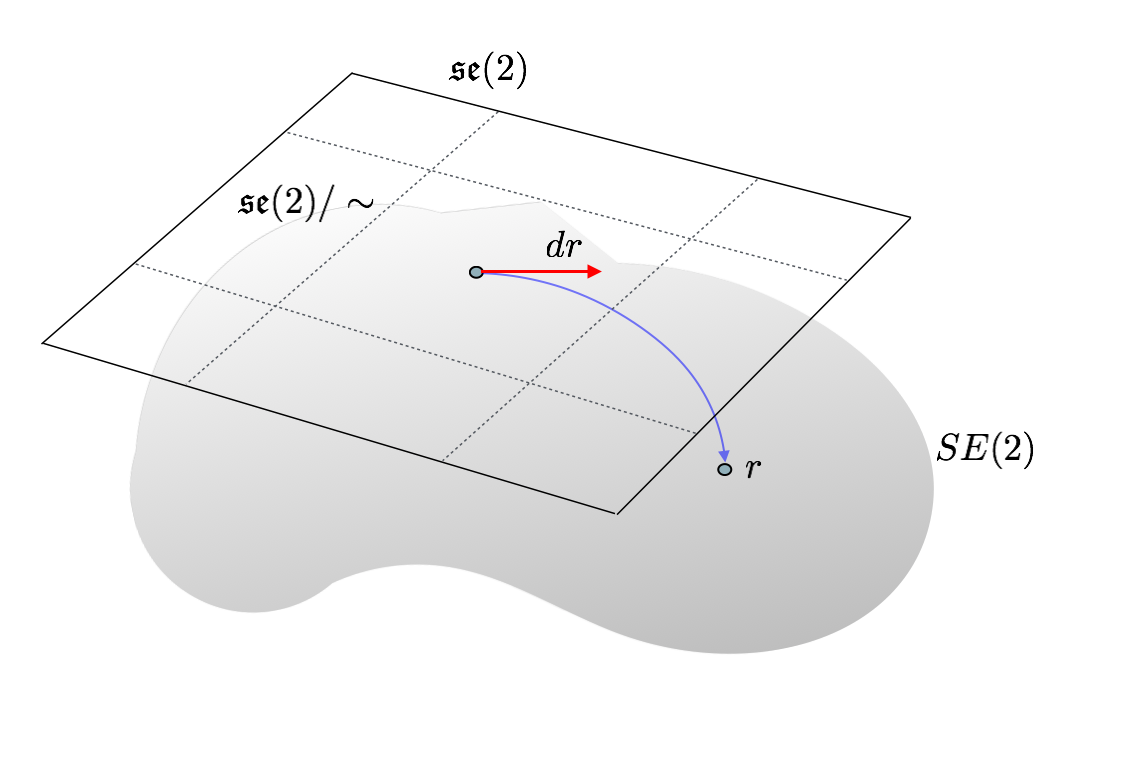
\includegraphics[scale=0.35]{figures/exp_se2.png}
		\caption{The Lie algebra $\mathfrak{se}(2)/\sim$ defined as the quotient of the Lie algebra $\mathfrak{se}(2)$ over the equivalence relation $\sim$ is in bijective correspondence with $SE(2)$.}
		\label{fig:restriction_exp_se2}
	\end{figure}
	
\end{enumerate}

% % % % % % % % % % % % % % % % % %
% % % % % % % % % % % % % % % % % % %
\subsection{Computations of Log-composition in SE(2)}
The log composition of two elements $dr_0 = (\theta_0, dr_{0x}, dr_{0y}), dr_1 = (\theta_1, dr_{1x}, dr_{1y})$ in $ \mathfrak{se}(2)/\sim$ is provided as a direct applications of the definitions provided for this case. It results
\begin{align*}
& dr_0 \oplus dr_1 =  \log(\exp(dr_0)\circ \exp(dr_1)) 
\end{align*}
for the computation of the ground truth.\\
The approximations of the log-composition using truncated BCH formulas are straightforward:
\begin{align*}
dr_0 \oplus dr_1 &\simeq  BCH^{0}(dr_0,dr_1 ) = dr_0 + dr_1  \\
dr_0 \oplus dr_1 &\simeq BCH^{1}(dr_0,dr_1 ) =  dr_0 + dr_1 + \frac{1}{2}[dr_0, dr_1] \\
dr_0 \oplus dr_1 &\simeq BCH^{2}(\mathbf{u},\mathbf{v}) =  dr_0 + dr_1 + \frac{1}{2}[dr_0, dr_1] + \frac{1}{12}([dr_0,[dr_0, dr_1]] + [dr_1,[dr_1, dr_0]] )
\end{align*}

To compute the approximation with the Taylor method, and so to compute the equation \ref{eq:taylor}, we observe that the vector form of the Lie bracket is given by
\begin{align*}
[dr_0, dr_1] &= (0, dR(\theta_0)dt_1 - dR(\theta_1)dt_0)^T \\
& = (0, -\theta_0 dr_{1y} + \theta_1 dr_{0y} ,  \theta_0 dr_{1x} - \theta_1 dr_{0x})^T
\end{align*} 
Therefore, the adjoint operator can be written in matrix form as a dual matrix of $dr$:
\begin{align*}
\text{ad}_{dr} = 
\left (
\begin{array} {c c c}
0            &  0        &      0\\
dr_y       &  0        & - \theta \\
- dr_x   & \theta &  0
\end{array}
\right )
\end{align*} 
In fact, when applied to $dr_1$ it results in the Lie bracket:
\begin{align*}
\text{ad}_{dr_0} dr_1= 
\left (
\begin{array} {c c c}
0            &  0        &      0\\
dr_{0y}       &  0        & - \theta_0 \\
- dr_{0x}   & \theta_0 &  0
\end{array}
\right )
\left (
\begin{array} {c }
\theta_1   \\
dt_{1x}    \\
dt_{1y}  
\end{array}
\right )
=
\left (
\begin{array} {c }
0  \\
-\theta_0 dt_{1y} + \theta_1 dt_{0y} \\ 
 \theta_0 dt_{1x} - \theta_1 dt_{0x} 
\end{array}
\right )
\end{align*} 
To compute the Taylor approximation proposed in equation \ref{eq:taylor} of the log composition, indicating $dt^{\star} = (dt_{y}, - dt_{x})$ it can be proved easily by induction that
\begin{align*}
\text{ad}_{dr}^{n} 
= 
\left (
\begin{array} {c c}
0            &  0        \\
dt^{\star}      &  dR(\theta)      
\end{array}
\right )^n
=
\left (
\begin{array} {c c}
0            &  0        \\
dR(\theta)^{n-1}dt^{\star}      &  dR(\theta)^{n}      
\end{array}
\right )
\end{align*}
And so the series involved in the equation $\ref{eq:taylor}$ become
\begin{align*}
\sum_{n=0}^{\infty} \frac{B_{n}}{n!} \text{ad}_{dr}^{ n} 
=
\sum_{n=0}^{\infty} \frac{B_{n}}{n!} \left (
\begin{array} {c c}
0            &  0        \\
dR(\theta)^{n-1}dt^{\star}      &  dR(\theta)^{n}      
\end{array}
\right ) 
\end{align*}
We can split it in two part, the rotational part and the translational part. The rotational part, using the nature of Bernoulli numbers and its generative equation, when $\theta \neq 0$ become
\begin{align*}
\sum_{n=0}^{\infty} \frac{B_{n}}{n!} dR(\theta)^{n}  
&=
I + \frac{1}{2}dR(\theta) + \sum_{n=1}^{\infty}\frac{B_{2n}}{2n!} dR(\theta)^{2n}  \\
&=
I + \frac{1}{2}dR(\theta) + (\sum_{n=1}^{\infty}\frac{B_{2n}}{2n!} (i \theta)^{2n})I  \\
&=
\frac{1}{2}dR(\theta) + (\sum_{n=0}^{\infty}\frac{B_{n}}{n!}(i \theta)^{n} - \frac{1}{2} i\theta) I  \\
&=
\frac{1}{2}dR(\theta) + (\sum_{n=0}^{\infty} \frac{i\theta e^{i\theta}}{e^{i\theta} - 1} - \frac{1}{2} i\theta) I  \\
&=
\frac{1}{2}dR(\theta) +  \frac{\theta /2}{\tan(\theta/2} I  
\end{align*}
while for the translational part
\begin{align*}
\sum_{n=1}^{\infty} \frac{B_{n}}{n!} dR(\theta)^{n-1} dt^{\star} 
&=
dR(\theta)^{-1} \Big(\sum_{n=1}^{\infty}\frac{B_{n}}{n!} dR(\theta)^{n}\Big)dt^{\star} \\
&=
dR(\theta)^{-1}  \Big(\sum_{n=0}^{\infty}\frac{B_{n}}{n!} dR(\theta)^{n} - I \Big)dt^{\star}  \\
&=
dR(\theta)^{-1}  \Big(\sum_{n=0}^{\infty} \frac{1}{2}dR(\theta) +  \frac{\theta /2}{\tan(\theta/2} I  - I \Big) dt^{\star} \\ 
&=
dR(\theta)^{-1}  \Big(\sum_{n=0}^{\infty} \frac{1}{2}dR(\theta) +  \frac{\theta /2}{\tan(\theta/2} I  - I \Big)dt^{\star} \\
&=
\Big(\frac{1}{2} I + (\frac{\theta /2}{\tan(\theta/2} - 1)dR(\theta)^{-1}   \Big) dt^{\star}    \\
\end{align*}
Finally the closed form for the Taylor approximation of the log-composition is \cite{vercauteren2014preprint}:
\begin{align}\label{eq:taylor_se2}
dr_{0}\oplus dr_{1}
=
dr_{0}
+
\sum_{n=0}^{\infty} \frac{B_{n}}{n!} \text{ad}_{dr_{0}}^{ n} 
dr_{1}
+
\mathcal{O}(dr_{1}^2)
=
dr_{0}
+
\mathbf{J}(dr_{0}, dr_{1})
dr_{1}
+
\mathcal{O}(dr_{1}^2)
\end{align}
where 
\begin{align*}
\mathbf{J}(dr_{0}, dr_{1})
=
\left (
\begin{array} {c c c}
1            &  0        &      0
\\
-\frac{\theta_0/2 - \tan(\theta_0/2)}{\theta_0\tan(\theta_0/2)}  dr_{0x} + \frac{1}{2}dr_{0y}       
&  \frac{\theta_0 /2}{\tan(\theta_0/2)} 
& - \theta_0/2 
\\
-  \frac{1}{2} dr_{0x} -\frac{\theta_0/2 - \tan(\theta_0/2)}{\theta_0\tan(\theta_0/2)} dr_{0y}       
& \theta_0/2 
&  \frac{\theta_0 /2}{\tan(\theta_0/2)}
\end{array}
\right )
\end{align*}

The approximation of the log-composition using parallel transport is a straightforward application of the equation \ref{eq:parallel_transport}: 
\begin{align}\label{eq:parallel_transport_se2}
dr_{0}\oplus dr_{1}
&\simeq
dr_{0}
+
\exp\big(\frac{dr_{0}}{2}\big)   
\exp(dr_{1}) 
\exp\big(-\frac{dr_{0}}{2}\big)
-
I
\end{align}
where the composition in the Lie group coincides with the product of matrix in the bigger algebra $GL(3)$ that contains both the Lie group $SE(2)$ and the Lie algebra $\mathfrak{se}(2)$.


% % % % % % % % % % % % % % % % % % % % % % % % % % % % % % % % % % % %
% % % % % % % % % % % % % % % % % % % % % % % % % % % % % % % % % % % %
% % % % % % % % % % % % % % % % % % % % % % % % % % % % % % % % % % % %
% % % % % % % % % % % % % % % % % % % % % % % % % % % % % % % % % % % %
\section{One-parameter Subgroup Generated by Stationary Velocity Fields}

As previously said, the passage from the finite to the infinite dimensional case is not free of deceptions. For the particular case of diffeomorphisms over the compact subset $\Omega\subset\mathbb{R}^d$, indicated with $\text{\emph{Diff}}(\Omega)$, the exponential map is not a local bijection (see the counterexample in \cite{lorenzi2013geodesics}, pag. 6 or the definition of Koppel-diffeomorphisms \cite{grabowski1988free} pag. 115). 
We will consider only the subset $G$ of $\text{\emph{Diff}}(\Omega)$ that are in the image of the exponential function $\exp$, or, in other world, the diffeomorphisms that belongs to the one-parameter subgroup.\\
If we indicate with $G$ the one-parameter subgroup of $\text{\emph{Diff}}(\Omega)$, each of the element of $G$ are generated by a tangent vector field in $\mathcal{C}^{\infty}(\Omega)$ (see definitions in subsection \ref{se:intro_lddmm}) toward an ODE (see \cite{arnold2006ordinary}). These generating tangent vector field can be divided into two classes that split the ODE in two classes:
\begin{enumerate}
	\item Stationary  - or homogeneous
	\begin{align*}
	\frac{d\varphi(t)}{dt} = V_{\varphi(t)}
	\end{align*}
	\item Non-stationary - or non-homogeneous
	\begin{align*}
	\frac{d\varphi(t)}{dt} = V_{(t, \varphi(t))}
	\end{align*}
\end{enumerate}
For a fixed $t$ both the stationary vector field (or SVF) $V_{\varphi(t)}$ and the time varying vector field (or TVVF) $V_{(t, \varphi(t))}$ belong to $G$. When varying $t$, the TVVFs behave as continuous paths over the tangent vector field, corresponding to the one-parameter subgroup $G$ through the map $\exp$.\\
Thanks to the Cauchy theorem that ensures the uniqueness of the solution of the ODE, under the initial condition $\varphi(0) = e$, the local bijection between $G$ and the Lie algebra of the tangent vector fields over $\Omega$ is ensured (see \cite{milnor1982infinite}, \cite{khesin2008geometry}):
\begin{align*}
\mathcal{V}(\Omega) \simeq  G \subset \text{Diff}(\Omega)
\end{align*}
and, as consequence of the definition of $\exp$ and $\log$ it follows that
\begin{align*}
G &= \exp( \mathcal{V}(\Omega))\\
\mathcal{V}(\Omega) &= \log(G)
\end{align*}
In the LDDMM framework only TVVFs were considered, while after \cite{arsigny2006log} only SVF has been considered for practical applications.\\
For our purposes when talking about diffeomorphisms, we will take into account only the one-parameter subgroup $G$, or in other world the image of a SVF through the $\exp$ map. 

% % % % % % % % % % % % % % % % % %
% % % % % % % % % % % % % % % % % % %
\subsection{Computations of Log-composition for SVF}
A closed-form for the Taylor Expansion method \ref{se:taylor_expansion} to compute the log-composition with SVF is not known. We will therefore compare the truncated BCH formula with the parallel transport method \ref{se:parallel_transport}. Since there is closed form for the log-composition, we will exploit the parametrization of discretized SVF using matrices to have a ground truth to compare results. Norm will be computed in the group as the $L_2$ norm of matrices that represents the SVF. \\ 
Given $\mathbf{u}$ and $\mathbf{v}$ SVF, $\mathbf{w}_{\text{ground}} = \mathbf{u}\oplus \mathbf{v}$ solution of the log-composition and $\mathbf{w}_{\text{app}}$ its approximation using a numerical method, then their difference is computed in the group as:
\begin{align*}
\text{error} = \euclideanMetric{\exp(\mathbf{w}_{\text{ground}}) - \exp(\mathbf{w}_{\text{app}})}_{L^{2}}
\end{align*}
where $\exp(\mathbf{w}_{\text{ground}})$ is computed as the composition of the exponentials of $\mathbf{u}$ and $\mathbf{v}$:
\begin{align*}
\exp(\mathbf{w}_{\text{ground}}) = \exp(\mathbf{u})\circ \exp(\mathbf{v})
\end{align*}
As previously said, the norm $L^2$ is meaningful in a group only because of the discrete implementation of the SVF in 5-dimensional matrices (see equation \ref{eq:basic_data_structure}).\\
(TODO: restate this in the limitations suggesting an alternative computation of the error as future work)\\


Further details about the methodology utilized to compare log-composition for SVF are provided in chapter \ref{ch:results}.






